% questions.tex —— 2010 年·普通高等学校招生考试·浙江卷·文科 · 题目内容片段（无答案）
% 由 tools/generate_projects.py 依来源总账自 2010/2010_数学真题_浙江文_试题.md 生成，勿手改（改源 MD 后重跑）
状态：needs-review；依固定候选 PDF 两页（印刷页 641–642）逐题核验，七幅图表已矢量重绘。原页未印分值，不补。
\gkpart{一、选择题}
\begin{question}
\gkti{1}设 $P=\{x\mid x<1\}$，$Q=\{x\mid x^2<4\}$，则 $P\cap Q=$（　）

（A）$\{x\mid -1<x<2\}$

（B）$\{x\mid -3<x<-1\}$

（C）$\{x\mid 1<x<4\}$

（D）$\{x\mid -2<x<1\}$

\end{question}
\begin{question}
\gkti{2}已知函数 $f(x)=\log_2(x+1)$，若 $f(\alpha)=1$，则 $\alpha=$（　）

（A）$0$

（B）$1$

（C）$2$

（D）$3$

\end{question}
\begin{question}
\gkti{3}设 $\mathrm i$ 为虚数单位，则 $\dfrac{5-\mathrm i}{1+\mathrm i}=$（　）

（A）$-2-3\mathrm i$

（B）$-2+3\mathrm i$

（C）$2-3\mathrm i$

（D）$2+3\mathrm i$

\Needspace{0.4\textheight}
\end{question}
\begingroup
\renewenvironment{question}{\Needspace{0.5\textheight}}{}
\begin{question}
\gkti{4}某程序框图如图所示，若输出的 $S=57$，则判断框内为（　）

（A）$k>4$?

（B）$k>5$?

（C）$k>6$?

（D）$k>7$?
\nopagebreak[4]
\begin{center}% 2010 年浙江卷文科第 4 题：程序框图（判断框内容待填）。
% 来源 PDF：普通高考/2010/2010浙江文.pdf，SHA-256 a73e22ea405697775b2d5cd82532fcffad0f506b849d9f199265b4297b8a754b。
% 原页：第 1 页（A3 三栏）第 1 栏中部，书页码 641。
% 重绘依据：照原页流程，开始→S=1,k=1→k=k+1→S=2S+k→判断框；
%   判断框“是”向下经“输出 S”到“结束”，“否”自左侧折回 k=k+1 上方。
\begin{tikzpicture}[scale=1.0, semithick,
  every node/.style={inner sep=2pt},
  box/.style={draw, minimum width=2.4cm, minimum height=0.58cm, align=center},
  round/.style={draw, rounded corners=5pt, minimum width=1.4cm,
    minimum height=0.58cm, align=center},
  para/.style={draw, trapezium, trapezium left angle=70, trapezium right angle=110,
    minimum width=2.2cm, minimum height=0.6cm, align=center},
  dec/.style={draw, diamond, aspect=2.2, minimum width=3.0cm,
    minimum height=1.15cm, align=center},
  arr/.style={->, >=stealth}]

  \node[round] (start) at (0,8.4) {开始};
  \node[box]   (init)  at (0,7.35) {$S=1,\ k=1$};
  \node[box]   (inc)   at (0,5.75) {$k=k+1$};
  \node[box]   (sum)   at (0,4.55) {$S=2S+k$};
  \node[dec]   (test)  at (0,3.05) {};
  \node[para]  (out)   at (0,1.75) {输出 $S$};
  \node[round] (end)   at (0,0.7)  {结束};

  \draw[arr] (start) -- (init);
  \draw[arr] (init) -- (inc);
  \draw[arr] (inc) -- (sum);
  \draw[arr] (sum) -- (test);
  \draw[arr] (test.south) -- (out.north);
  \node[right] at (0.12,2.35) {是};
  \draw[arr] (out) -- (end);
  \draw[arr] (test.west) -- (-2.35,3.05) -- (-2.35,6.55) -- (0,6.55);
  \node[left] at (-2.5,3.2) {否};
\end{tikzpicture}
\end{center}
\nopagebreak[4]
\end{question}
\endgroup
\begin{question}
\gkti{5}设 $S_n$ 为等比数列 $\{a_n\}$ 的前 $n$ 项和，$8a_2+a_5=0$，则 $\dfrac{S_5}{S_2}=$（　）

（A）$-11$

（B）$-8$

（C）$5$

（D）$11$

\end{question}
\begin{question}
\gkti{6}设 $0<x<\dfrac{\pi}{2}$，则“$x\sin^2x<1$”是“$x\sin x<1$”的（　）

（A）充分而不必要条件

（B）必要而不充分条件

（C）充分必要条件

（D）既不充分也不必要条件

\end{question}
\begingroup
\renewenvironment{question}{\Needspace{0.4\textheight}}{}
\begin{question}
\gkti{7}若实数 $x$，$y$ 满足不等式组
\nopagebreak[4]
\[\begin{cases}
x+3y-3\geqslant 0,\\
2x-y-3\leqslant 0,\\
x-y+1\geqslant 0,
\end{cases}\]
则 $x+y$ 的最大值为（　）

（A）$9$

（B）$\dfrac{15}{7}$

（C）$1$

（D）$\dfrac{7}{15}$

\Needspace{0.4\textheight}
\end{question}
\endgroup
\begingroup
\renewenvironment{question}{\Needspace{0.5\textheight}}{}
\begin{question}
\gkti{8}若某几何体的三视图（单位：cm）如图所示，则此几何体的体积是（　）

（A）$\frac{352}{3}\ \mathrm{cm}^3$

（B）$\frac{320}{3}\ \mathrm{cm}^3$

（C）$\frac{224}{3}\ \mathrm{cm}^3$

（D）$\frac{160}{3}\ \mathrm{cm}^3$
\nopagebreak[4]
\begin{center}% 2010 年浙江卷文科第 8 题：三视图（正视图、侧视图、俯视图）。
% 来源 PDF：普通高考/2010/2010浙江文.pdf，SHA-256 a73e22ea405697775b2d5cd82532fcffad0f506b849d9f199265b4297b8a754b。
% 原页：第 1 页（A3 三栏）第 2 栏上部，书页码 641。
% 重绘依据：正视图与侧视图均为下底 8、上底 4、高 2 的等腰梯形，其上叠 4×2 的矩形；
%   俯视图为外方 8×8、内方 4×4、四角以对角线相连。尺寸 2、4、2 与 2、2 照原页标注。
\begin{tikzpicture}[scale=0.45, semithick, every node/.style={inner sep=1.5pt, font=\small},
  dim/.style={<->, >=stealth, thin}]

  % ---------- 正视图 ----------
  \draw (-4,0) -- (4,0) -- (2,2) -- (-2,2) -- cycle;
  \draw (-2,2) rectangle (2,4);
  % 顶部尺寸 2,4,2
  \draw[thin] (-4,4.25) -- (-4,4.85);
  \draw[thin] (-2,4.25) -- (-2,4.85);
  \draw[thin] (2,4.25) -- (2,4.85);
  \draw[thin] (4,4.25) -- (4,4.85);
  \draw[dim] (-4,4.55) -- (-2,4.55);
  \draw[dim] (-2,4.55) -- (2,4.55);
  \draw[dim] (2,4.55) -- (4,4.55);
  \node[above] at (-3,4.55) {$2$};
  \node[above] at (0,4.55) {$4$};
  \node[above] at (3,4.55) {$2$};
  % 右侧尺寸 2,2
  \draw[thin] (4.15,4) -- (4.75,4);
  \draw[thin] (4.15,2) -- (4.75,2);
  \draw[thin] (4.15,0) -- (4.75,0);
  \draw[dim] (4.45,2) -- (4.45,4);
  \draw[dim] (4.45,0) -- (4.45,2);
  \node[right] at (4.45,3) {$2$};
  \node[right] at (4.45,1) {$2$};
  \node[below] at (0,-0.9) {正视图};

  % ---------- 侧视图 ----------
  \begin{scope}[shift={(11,0)}]
    \draw (-4,0) -- (4,0) -- (2,2) -- (-2,2) -- cycle;
    \draw (-2,2) rectangle (2,4);
    \node[below] at (0,-0.9) {侧视图};
  \end{scope}

  % ---------- 俯视图 ----------
  \begin{scope}[shift={(0,-3.4)}]
    \draw (-4,0) rectangle (4,-8);
    \draw (-2,-2) rectangle (2,-6);
    \draw (-4,0) -- (-2,-2);
    \draw (4,0) -- (2,-2);
    \draw (4,-8) -- (2,-6);
    \draw (-4,-8) -- (-2,-6);
    % 右侧尺寸 2,4,2
    \draw[thin] (4.15,0) -- (4.75,0);
    \draw[thin] (4.15,-2) -- (4.75,-2);
    \draw[thin] (4.15,-6) -- (4.75,-6);
    \draw[thin] (4.15,-8) -- (4.75,-8);
    \draw[dim] (4.45,-2) -- (4.45,0);
    \draw[dim] (4.45,-6) -- (4.45,-2);
    \draw[dim] (4.45,-8) -- (4.45,-6);
    \node[right] at (4.45,-1) {$2$};
    \node[right] at (4.45,-4) {$4$};
    \node[right] at (4.45,-7) {$2$};
    \node[below] at (0,-8.9) {俯视图};
  \end{scope}
\end{tikzpicture}
\end{center}
\nopagebreak[4]
\end{question}
\endgroup
\begin{question}
\gkti{9}已知 $x_0$ 是函数 $f(x)=2^x+\dfrac{1}{1-x}$ 的一个零点。若 $x_1\in(1,x_0)$，$x_2\in(x_0,+\infty)$，则（　）

（A）$f(x_1)<0$，$f(x_2)<0$

（B）$f(x_1)<0$，$f(x_2)>0$

（C）$f(x_1)>0$，$f(x_2)<0$

（D）$f(x_1)>0$，$f(x_2)>0$

\end{question}
\begin{question}
\gkti{10}设 $O$ 为坐标原点，$F_1$，$F_2$ 是双曲线 $\dfrac{x^2}{a^2}-\dfrac{y^2}{b^2}=1$（$a>0$，$b>0$）的焦点。若在双曲线上存在点 $P$，满足 $\angle F_1PF_2=60^\circ$，$|OP|=\sqrt7a$，则该双曲线的渐近线方程为（　）

（A）$x\pm\sqrt3y=0$

（B）$\sqrt3x\pm y=0$

（C）$x\pm\sqrt2y=0$

（D）$\sqrt2x\pm y=0$

\end{question}
\gkpart{二、填空题}
\Needspace{0.4\textheight}
\begingroup
\renewenvironment{question}{\Needspace{0.5\textheight}}{}
\begin{question}
\gkti{11}在如图所示的茎叶图中，甲、乙两组数据的中位数分别是 $\underline{\qquad}$，$\underline{\qquad}$。
\nopagebreak[4]
\begin{center}% 2010 年浙江卷文科第 11 题：甲、乙两组数据的茎叶图。
% 来源 PDF：普通高考/2010/2010浙江文.pdf，SHA-256 a73e22ea405697775b2d5cd82532fcffad0f506b849d9f199265b4297b8a754b。
% 原页：第 1 页（A3 三栏）第 2 栏中部，书页码 641。
% 重绘依据：照原页布局，中间一列为公共茎，左为甲组叶、右为乙组叶；
%   茎自上而下为 2、3、4、5、6，叶按原页自左至右逐字照录（甲 8｜9 1｜2 5｜7 8 5｜6；
%   乙 9｜5 5｜8 2 6｜3 5｜7），两列竖线夹住茎列，表头上方一条横线。
\begin{tikzpicture}[scale=1.0, semithick, every node/.style={inner sep=1.5pt, font=\small}]

  % 表头与框线
  \node at (-1.0,0.8) {甲};
  \node at (1.5,0.8) {乙};
  \draw (-2.05,0.42) -- (2.4,0.42);
  \draw (0,0.42) -- (0,-2.55);
  \draw (0.62,0.42) -- (0.62,-2.55);

  % 第 1 行：茎 2
  \node at (0.31,0) {2};
  \node[anchor=east] at (-0.14,0) {8};
  \node[anchor=west] at (0.76,0) {9};

  % 第 2 行：茎 3
  \node at (0.31,-0.55) {3};
  \node[anchor=east] at (-0.48,-0.55) {9};
  \node[anchor=east] at (-0.14,-0.55) {1};
  \node[anchor=west] at (0.76,-0.55) {5};
  \node[anchor=west] at (1.10,-0.55) {5};

  % 第 3 行：茎 4
  \node at (0.31,-1.1) {4};
  \node[anchor=east] at (-0.48,-1.1) {2};
  \node[anchor=east] at (-0.14,-1.1) {5};
  \node[anchor=west] at (0.76,-1.1) {8};
  \node[anchor=west] at (1.10,-1.1) {2};
  \node[anchor=west] at (1.44,-1.1) {6};

  % 第 4 行：茎 5
  \node at (0.31,-1.65) {5};
  \node[anchor=east] at (-0.82,-1.65) {7};
  \node[anchor=east] at (-0.48,-1.65) {8};
  \node[anchor=east] at (-0.14,-1.65) {5};
  \node[anchor=west] at (0.76,-1.65) {3};
  \node[anchor=west] at (1.10,-1.65) {5};

  % 第 5 行：茎 6
  \node at (0.31,-2.2) {6};
  \node[anchor=east] at (-0.14,-2.2) {6};
  \node[anchor=west] at (0.76,-2.2) {7};
\end{tikzpicture}
\end{center}
\nopagebreak[4]
\end{question}
\endgroup
\begin{question}
\gkti{12}函数 $f(x)=\sin^2\left(2x-\dfrac{\pi}{4}\right)$ 的最小正周期是 $\underline{\qquad}$。

\end{question}
\begin{question}
\gkti{13}已知平面向量 $\boldsymbol\alpha$，$\boldsymbol\beta$ 满足 $|\boldsymbol\alpha|=1$，$|\boldsymbol\beta|=2$，$\boldsymbol\alpha\perp(\boldsymbol\alpha-2\boldsymbol\beta)$，则 $|2\boldsymbol\alpha+\boldsymbol\beta|$ 的值是 $\underline{\qquad}$。

\Needspace{0.4\textheight}
\end{question}
\begingroup
\renewenvironment{question}{\Needspace{0.5\textheight}}{}
\begin{question}
\gkti{14}在如下数表中，已知每行、每列中的数都成等差数列。
\nopagebreak[4]
\begin{center}% 2010 年浙江卷文科第 14 题：各行、各列都成等差数列的数表。
% 来源 PDF：普通高考/2010/2010浙江文.pdf，SHA-256 a73e22ea405697775b2d5cd82532fcffad0f506b849d9f199265b4297b8a754b。
% 原页：第 1 页（A3 三栏）第 2 栏下部，书页码 641。
% 重绘依据：照原页全框格排版，表头一行为“第 1 列、第 2 列、第 3 列、⋯”，
%   行标为“第 1 行、第 2 行、第 3 行、⋯”，格内数字 1 2 3 / 2 4 6 / 3 6 9，末行末列为省略号。
\begin{tikzpicture}[scale=0.9, semithick, every node/.style={inner sep=1pt, font=\small}]

  % 竖线
  \foreach \x in {0, 1.95, 3.5, 5.05, 6.6, 7.7} {
    \draw (\x,0.66) -- (\x,-2.64);
  }
  % 横线
  \foreach \y in {0.66, 0, -0.66, -1.32, -1.98, -2.64} {
    \draw (0,\y) -- (7.7,\y);
  }

  % 表头
  \node at (0.975,0.33) {第 $1$ 列};
  \node at (2.725,0.33) {第 $2$ 列};
  \node at (4.275,0.33) {第 $3$ 列};
  \node at (6.05,0.33) {$\cdots$};

  % 第 1 行
  \node at (0.975,-0.33) {第 $1$ 行};
  \node at (2.725,-0.33) {1};
  \node at (4.275,-0.33) {2};
  \node at (5.825,-0.33) {3};
  \node at (7.15,-0.33) {$\cdots$};

  % 第 2 行
  \node at (0.975,-0.99) {第 $2$ 行};
  \node at (2.725,-0.99) {2};
  \node at (4.275,-0.99) {4};
  \node at (5.825,-0.99) {6};
  \node at (7.15,-0.99) {$\cdots$};

  % 第 3 行
  \node at (0.975,-1.65) {第 $3$ 行};
  \node at (2.725,-1.65) {3};
  \node at (4.275,-1.65) {6};
  \node at (5.825,-1.65) {9};
  \node at (7.15,-1.65) {$\cdots$};

  % 末行
  \node at (0.975,-2.31) {$\cdots$};
  \node at (2.725,-2.31) {$\cdots$};
  \node at (4.275,-2.31) {$\cdots$};
  \node at (5.825,-2.31) {$\cdots$};
  \node at (7.15,-2.31) {$\cdots$};
\end{tikzpicture}
\end{center}
\nopagebreak[4]
那么，位于表中的第 $n$ 行第 $n+1$ 列的数是 $\underline{\qquad}$。

\end{question}
\endgroup
\begin{question}
\gkti{15}若正实数 $x$，$y$ 满足 $2x+y+6=xy$，则 $xy$ 的最小值是 $\underline{\qquad}$。

\end{question}
\begin{question}
\gkti{16}某商家一月份至五月份累计销售额达 $3860$ 万元，预测六月份销售额为 $500$ 万元，七月份销售额比六月份递增 $x\%$，八月份销售额比七月份递增 $x\%$，九、十月份销售总额与七、八月份销售总额相等。若一月至十月份销售总额至少达 $7000$ 万元，则 $x$ 的最小值是 $\underline{\qquad}$。

\Needspace{0.4\textheight}
\end{question}
\begingroup
\renewenvironment{question}{\Needspace{0.5\textheight}}{}
\begin{question}
\gkti{17}在平行四边形 $ABCD$ 中，$O$ 是 $AC$ 与 $BD$ 的交点，$P$，$Q$，$M$，$N$ 分别是线段 $OA$，$OB$，$OC$，$OD$ 的中点。在 $A$，$P$，$M$，$C$ 中任取一点记为 $E$，在 $B$，$Q$，$N$，$D$ 中任取一点记为 $F$。设 $G$ 为满足向量 $\overrightarrow{OG}=\overrightarrow{OE}+\overrightarrow{OF}$ 的点，则在上述的点 $G$ 组成的集合中的点，落在平行四边形 $ABCD$ 外（不含边界）的概率为 $\underline{\qquad}$。
\nopagebreak[4]
\begin{center}% 2010 年浙江卷文科第 17 题：平行四边形 ABCD，O 为对角线交点，
% P、Q、M、N 分别为 OA、OB、OC、OD 的中点。
% 来源 PDF：普通高考/2010/2010浙江文.pdf，SHA-256 a73e22ea405697775b2d5cd82532fcffad0f506b849d9f199265b4297b8a754b。
% 原页：第 1 页（A3 三栏）第 3 栏中部，书页码 641。
% 重绘依据：照原页，A 左上、B 右上、D 左下、C 右下；对角线 AC、BD 交于 O；
%   P 在 OA 上、Q 在 OB 上、M 在 OC 上、N 在 OD 上，四点均以实心点标出。
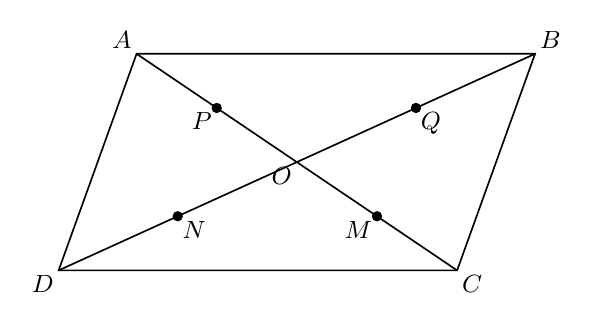
\begin{tikzpicture}[scale=1.1, semithick, every node/.style={inner sep=1.5pt, font=\small}]
  \coordinate (A) at (0.9,3.1);
  \coordinate (B) at (5.5,3.1);
  \coordinate (C) at (4.6,0.6);
  \coordinate (D) at (0,0.6);
  \coordinate (O) at (2.75,1.85);
  \coordinate (P) at (1.825,2.475);
  \coordinate (Q) at (4.125,2.475);
  \coordinate (M) at (3.675,1.225);
  \coordinate (N) at (1.375,1.225);

  \draw (A) -- (B) -- (C) -- (D) -- cycle;
  \draw (A) -- (C);
  \draw (B) -- (D);

  \fill (P) circle (1.7pt);
  \fill (Q) circle (1.7pt);
  \fill (M) circle (1.7pt);
  \fill (N) circle (1.7pt);

  \node[above left] at (A) {$A$};
  \node[above right] at (B) {$B$};
  \node[below right] at (C) {$C$};
  \node[below left] at (D) {$D$};
  \node[below left] at (O) {$O$};
  \node[below left] at (P) {$P$};
  \node[below right] at (Q) {$Q$};
  \node[below left] at (M) {$M$};
  \node[below right] at (N) {$N$};
\end{tikzpicture}
\end{center}
\nopagebreak[4]
\end{question}
\endgroup
\gkpart{三、解答题}
\begin{question}
\gkti{18}在 $\triangle ABC$ 中，角 $A$，$B$，$C$ 所对的边分别为 $a$，$b$，$c$。设 $S$ 为 $\triangle ABC$ 的面积，满足 $S=\dfrac{\sqrt3}{4}(a^2+b^2-c^2)$。

（1）求角 $C$ 的大小；

（2）求 $\sin A+\sin B$ 的最大值。

\end{question}
\begin{question}
\gkti{19}设 $a_1$，$d$ 为实数，首项为 $a_1$，公差为 $d$ 的等差数列 $\{a_n\}$ 的前 $n$ 项和为 $S_n$，满足 $S_5S_6+15=0$。

（1）若 $S_5=5$，求 $S_6$ 及 $a_1$；

（2）求 $d$ 的取值范围。

\Needspace{0.4\textheight}
\end{question}
\begingroup
\renewenvironment{question}{\Needspace{0.5\textheight}}{}
\begin{question}
\gkti{20}如图，在平行四边形 $ABCD$ 中，$AB=2BC$，$\angle ABC=120^\circ$。$E$ 为线段 $AB$ 的中点，将 $\triangle ADE$ 沿直线 $DE$ 翻折成 $\triangle A'DE$，使平面 $A'DE\perp$ 平面 $BCD$，$F$ 为线段 $A'C$ 的中点。

（1）求证：$BF\parallel$ 平面 $A'DE$；

（2）设 $M$ 为线段 $DE$ 的中点，求直线 $FM$ 与平面 $A'DE$ 所成角的余弦值。
\nopagebreak[4]
\begin{center}% 2010 年浙江卷文科第 20 题：平行四边形 ABCD 沿 DE 翻折成 △A'DE（透视示意）。
% 来源 PDF：普通高考/2010/2010浙江文.pdf，SHA-256 a73e22ea405697775b2d5cd82532fcffad0f506b849d9f199265b4297b8a754b。
% 原页：第 2 页（A3 三栏）第 1 栏下部，书页码 642。
% 重绘依据：照原页透视，A 左下、E 在 AB 中点、B 右下、D 左、C 右、A' 在上；
%   F 为 A'C 中点、M 为 DE 中点。原页虚线为 D–C 与 M–F，其余（AE、EB、AD、DE、
%   A'D、A'E、A'C、BC、BF）均为实线。
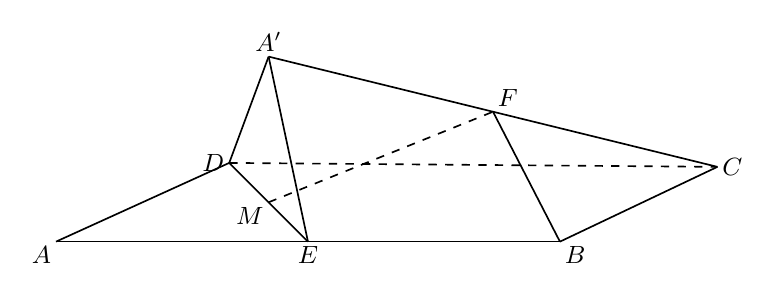
\begin{tikzpicture}[scale=1.0, semithick, every node/.style={inner sep=1.5pt, font=\small}]
  \coordinate (A)  at (0,0);
  \coordinate (E)  at (3.2,0);
  \coordinate (B)  at (6.4,0);
  \coordinate (D)  at (2.2,1.0);
  \coordinate (C)  at (8.4,0.95);
  \coordinate (Ap) at (2.7,2.35);
  \coordinate (F)  at (5.55,1.65);
  \coordinate (M)  at (2.7,0.5);

  % 底面与侧面
  \draw (A) -- (E) -- (B);
  \draw (A) -- (D);
  \draw (D) -- (E);
  \draw (B) -- (C);

  % 翻折后的三角形
  \draw (Ap) -- (D);
  \draw (Ap) -- (E);
  \draw (Ap) -- (C);
  \draw (B) -- (F);

  % 虚线：被遮挡的 D–C 与线段 M–F
  \draw[dashed] (D) -- (C);
  \draw[dashed] (M) -- (F);

  \node[above] at (Ap) {$A'$};
  \node[above right] at (F) {$F$};
  \node[below left] at (A) {$A$};
  \node[below] at (E) {$E$};
  \node[below right] at (B) {$B$};
  \node[left] at (D) {$D$};
  \node[right] at (C) {$C$};
  \node[below left] at (M) {$M$};
\end{tikzpicture}
\end{center}
\nopagebreak[4]
\end{question}
\endgroup
\begin{question}
\gkti{21}已知函数 $f(x)=(x-a)^2(x-b)$（$a$，$b\in\mathbf R$，$a<b$）。

（1）当 $a=1$，$b=2$ 时，求曲线 $y=f(x)$ 在点 $(2,f(2))$ 处的切线方程；

（2）设 $x_1$，$x_2$ 是 $f(x)$ 的两个极值点，$x_3$ 是 $f(x)$ 的一个零点，且 $x_3\neq x_1$，$x_3\neq x_2$。证明：存在实数 $x_4$，使得 $x_1$，$x_2$，$x_3$，$x_4$ 按某种顺序排列后成等差数列，并求 $x_4$。

\Needspace{0.4\textheight}
\end{question}
\begingroup
\renewenvironment{question}{\Needspace{0.5\textheight}}{}
\begin{question}
\gkti{22}已知 $m$ 是非零实数，抛物线 $C:y^2=2px$（$p>0$）的焦点 $F$ 在直线 $l:x-my-\dfrac{m^2}{2}=0$ 上。

（1）若 $m=2$，求抛物线 $C$ 的方程；

（2）设直线 $l$ 与抛物线 $C$ 交于 $A$，$B$ 两点，过 $A$，$B$ 分别作抛物线 $C$ 的准线的垂线，垂足为 $A_1$，$B_1$，$\triangle AA_1F$，$\triangle BB_1F$ 的重心分别为 $G$，$H$。求证：对任意非零实数 $m$，抛物线 $C$ 的准线与 $x$ 轴的交点在以线段 $GH$ 为直径的圆外。
\nopagebreak[4]
\begin{center}% 2010 年浙江卷文科第 22 题：抛物线 C、准线、焦点 F，以及 △AA_1F、△BB_1F 的重心 G、H。
% 来源 PDF：普通高考/2010/2010浙江文.pdf，SHA-256 a73e22ea405697775b2d5cd82532fcffad0f506b849d9f199265b4297b8a754b。
% 原页：第 2 页（A3 三栏）第 3 栏上部，书页码 642。
% 重绘依据：照原页，抛物线开口向右、顶点在原点 O；准线为左侧竖直线，
%   A_1、B_1 在准线上且 A_1A、B_1B 水平；弦 AB 过焦点 F（即直线 l）；
%   连 A_1F、B_1F，标出重心 G、H（原页无圆，只标两点）。
%   题设 p=m^2，取 m=0.35（p=0.1225）并按 p/2 归一化作图，得 y^2=4x、准线 x=-1、
%   F(1,0)、A(1.99,2.82)、B(0.50,-1.42)、G(0.66,1.88)、H(0.17,-0.95)。
\begin{tikzpicture}[scale=1.05, semithick, every node/.style={inner sep=1.2pt, font=\small}]

  % 抛物线 y^2 = 4x，即 x = y^2/4
  \draw[domain=-1.55:3.0, samples=160, smooth, variable=\y]
    plot ({(\y*\y)/4}, \y);

  % 坐标轴
  \draw[->, >=stealth] (-1.3,0) -- (3.9,0);
  \draw[->, >=stealth] (0,-1.6) -- (0,3.05);
  \node[below right] at (3.9,0) {$x$};
  \node[left] at (0,3.05) {$y$};

  % 准线
  \draw (-1,-1.5) -- (-1,2.95);

  % 关键点
  \coordinate (A1) at (-1,2.82);
  \coordinate (B1) at (-1,-1.42);
  \coordinate (A)  at (1.99,2.82);
  \coordinate (B)  at (0.50,-1.42);
  \coordinate (F)  at (1,0);
  \coordinate (G)  at (0.663,1.88);
  \coordinate (H)  at (0.167,-0.947);

  % 水平投影线与连线
  \draw (A1) -- (A);
  \draw (B1) -- (B);
  \draw (A1) -- (F);
  \draw (B1) -- (F);
  \draw (A) -- (B);

  \fill (G) circle (1.7pt);
  \fill (H) circle (1.7pt);

  \node[left] at (A1) {$A_1$};
  \node[left] at (B1) {$B_1$};
  \node[above left] at (A) {$A$};
  \node[below right] at (B) {$B$};
  \node[below right] at (F) {$F$};
  \node[below left] at (0,0) {$O$};
  \node[left] at (G) {$G$};
  \node[right] at ($(H)+(0.06,0.09)$) {$H$};
\end{tikzpicture}
\end{center}
\nopagebreak[4]

\end{question}
\endgroup